\def\mytitle{Whirlwind: Overload protection, fault--tolerance and self--tuning in an Internet services platform}
\def\myauthor{Peter Donald, Samar Singh and Somnath Ghosh}
\def\mykeywords{concurrency}

\documentclass[conference]{IEEEtran}

\usepackage{cite}
\usepackage[pdftex]{graphicx,hyperref}
\usepackage{url}
\usepackage{epstopdf}

\pdfinfo{/Title (\mytitle) 
         /Author (\myauthor)
         /Keywords (\mykeywords)}

\newcommand{\todo}[1]{{\bf\begin{center}TODO: #1\end{center}}}

\begin{document}

\title{\mytitle}

\author{\IEEEauthorblockN{\myauthor}
\IEEEauthorblockA{School of Computer Science and Electronic Engineering\\
La Trobe University,\\
Melbourne, Australia\\
Email: peter@realityforge.org, S.Singh@latrobe.edu.au and S.Ghosh@latrobe.edu.au}
}

\maketitle

\begin{abstract}
Performance and availability are critical importance when Internet services are integrated into emergency response management. Poor performance or service failure can result in severe economic, social or environmental cost. This paper presents Whirlwind, a software architecture that includes primitives for overload management and fault tolerance. A Whirlwind service is composed of a collection of isolated, independent, sequential processes that communicate through asynchronous message passing. If a process fails, the fault is contained within the process and a message is propagated to monitoring processes that may attempt to recover from the error. Processes are grouped with other processes that share similar resource, computation and concurrency requirements. Each group contains a scheduler and a thread pool that drives execution of processes within the group. The group may also define a message predicate that determines if a message posted to a process in the group is accepted. A rejected message typically signals overload and allows the application the chance to perform load shedding and avoid overcommitment of resources. Principles are shared between processes in different groups, enabling consistent prioritization and admission control across groups. The resource management policies are typically driven by feedback loops that monitor resource availability and system performance, and adjust tuning parameters to meet performance goals. Whirlwind evolved over a period of five fire seasons as part of emergency response software in Victoria, Australia.
\end{abstract}

\IEEEpeerreviewmaketitle

\section{Introduction}

Whirlwind was born out of the need to create a reliable, scalable software architecture for the Incident Resource Information System (IRIS). IRIS tracks the dispatch and deployment of resources during an emergency situation. The resources include everything from vehicles to personnel and the emergency situations have included wildfires, floods and virus outbreaks. IRIS is also responsible for generating the payments for personnel during emergency situations.

%When data is updated in an \emph{area}, the data is replicated to clients who have subscribed to that particular \emph{area}. During emergency situations the data churn tends to be restricted to specific areas that correspond to geographic locations that the emergency occurred in and most clients have subscribed to that particular area. This typically results in a load that grows exponentially with respect to the number of concurrent users. 

Internet traffic is bursty~\cite{Crovella:1996:BurstyTraffic} and popular Internet services are likely to be subject to periods of transient or sustained overload. This is intensified for Internet services used in emergency responses. Overload can be caused by unexpectedly high request rates or unexpected shifts in the characteristics of the request distribution. In IRIS the request rate increased dramatically during shift change over times or prior to payment cut--off dates. The characteristics of the requests also changed dramatically depending on whether the users were primarily interacting with payment subsystem or the resource tracking subsystem.

During periods of overload, many services suffer from response time spikes, throughput loss, unpredictable behavior and crashing. During the February 2009 Victorian bushfires, the number of concurrent users was 5x greater than during previous emergencies. In IRIS, the load grows exponentially with respect to the number of concurrent users and this resulted in a rapid, dramatic, unanticipated increase in system load. Over--provisioning the service can only alleviate the pressure, not avoid the overload problem altogether. 
 
Whirlwind is based on the actor model of concurrency. It incorporates existing work on load management, fault--tolerance, scheduling and self--tuning and synthesizes these elements into a consistent framework. Whirlwind was developed for the Java Virtual Machine, principally targeting the Java programming language. The architecture needed to take advantage of the increased number of processing units in modern hardware.

Early in the evolution of Whirlwind it was discovered that it was necessary to provide flexibility in certain aspects such as admission control policies and scheduling algorithms. Plugin points are defined where flexibility was required. To maintain acceptable performance the plugins are designed with coarse--grain interfaces with minimal virtual calls along critical paths. 

Included with Whirlwind is an library designed to evaluate and report the performance of Whirlwind applications while avoiding many of the common pitfalls of Java performance evaluation~\cite{Blackburn:EvaluationMethodology,Georges:JavaPerformance}. Part of the goal was to compare different versions of Whirlwind but it is also useful in evaluating a Whirlwind application.

Each iteration of Whirlwind has undergone an extensive performance evaluation before being rolled out into production. Space does not permit presenting a a detailed performance report. Suffice to say that Whirlwind, at least with certain plugins configured, met the original performance goals and compares favorably with other popular production frameworks.

\section{Background Material}

Past research has focused on parts of the problem but there has been no attempt to bring all the elements together in one consistent framework. A single platform makes it possible to compare the techniques in various combinations and configurations and isolate variation due to environmental factors.

\subsection{Load Management}

Previous work on load management has focused on using techniques such as admission control~\cite{Voigt:2001qe,Cherkasova:2002yb,srinivas00webk,Kanodia:2000qv,welsh03Adaptive,Elnikety:2004ty}, service degradation~\cite{welsh03Adaptive,abdelzaher99web} and scheduling policies~\cite{Zhou06RequestAware,Behren03Capriccio,Schroeder06Overload,Crovella99Alpha,Cherkasova1998Strategy,Larus:2002:Cohort} to limit response time spikes and maintain throughput during periods of overload. Admission control rejects a subset of requests so that the remaining requests meet response time goals. Service degradation aims to deliver less resource intensive content during periods of overload. The assumption is that it is better to deliver some content on time rather than fail to deliver the full content on time, or at all. Scheduling policies determine the order in which requests are accepted and after they have been accepted, the policy for sharing the available processor resources.

Load shedding is typically achieved by selectively applying the above techniques to different requests. Requests can be categorized by low level connection properties~\cite{Voigt:2001qe}, protocol specific parameters (i.e. the url, headers or session associated with a HTTP request)~\cite{Cherkasova:2002yb,Voigt:2001qe} or application specific metrics (i.e. revenue and profits~\cite{Menasec:2000ty}, or \emph{Premium} vs \emph{Basic} users). Requests can also be categorized according to the expected change in resource availability after processing request~\cite{Behren03Capriccio} or predicted resource cost to process request~\cite{Crovella99Alpha}. Other systems categorize the request based on estimated utility\cite{Zhou06RequestAware} or ability to meet performance goals (i.e. the 90th--percentile of response time~\cite{welsh03Adaptive}). Class--based differentiation is a coarse--grain classification scheme but fine--grain classification schemes are common.

Past research has tended to focus one categorization axis rather than categorizing a request along multiple dimensions. It is probable that this is done as it makes the mapping between a categorization and a priority simple; \emph{Premium} users are always prioritized above \emph{Basic} users, \emph{Buy} requests are always prioritized above \emph{Browse} requests, while during overload light--weight requests are always prioritized above heavy--weight requests etc. 

\subsection{Fault Tolerance}

%Faults occur, yet most systems are not designed to expect faults and limit the impact of faults when they occur. Fault tolerant systems must be able to isolate faults, detect a fault has occurred and reinitialize a subsystem after it fails from some known good state~\cite{Schneider:FailStopProcessors}. The system can then retry the operation that lead to the failure. Shared memory architectures can not isolate faults thus limiting fault tolerance within the application~\cite{Armstrong03Thesis}.

A fault tolerant system is one ``\ldots able to recover from errors and to restore normal operation \ldots''~\cite{Renzel:03:ErrorHandling} If there is a decrease in service quality, the degradation is proportional to the severity of the fault. Fault tolerance is achieved by expecting faults and designing the system so that it behaves reasonably in the presence of faults.

The Tandem NonStop system has a mean time between failures measured in years~\cite{Grey85Fail} and indirectly influenced many of the design decisions of Whirlwind. The architecture consists of hierarchically decomposing a system into processes where each process is a single unit of service and a single unit of failure. Processes share no state and only communicate via messages. A failure in a process does not propagate to other processes thus resulting in fault containment. The system was also designed using a fail--fast philosophy so that processes either function correctly or detect the fault, signal failure and stop operation.

The construction of fault--tolerant computing systems is simplified when programs do not need to cope with arbitrary behavior or corrupted state information. So not only should a failure be contained within a process, but on detection of a failure the process should halt rather than make erroneous state visible to other processors. Other processors should be able to detect if a process has failed so that they can attempt error recovery. Error recovery should have a known good state with which to restart the process. Similar properties are deemed necessary to construct fault--tolerant hardware systems~\cite{Schneider:FailStopProcessors}.  

Erlang is a software architecture designed to survive software and hardware faults~\cite{Armstrong03Thesis} and incorporates these strategies. Erlang models the world as isolated processes. When a process terminates either normally or due to failure, a message is sent to all monitoring processes. The monitoring processes can then take action to recover from the error if required.

An Erlang supervisor is a process that monitors child processes. If a child process fails, the supervisor uses a \emph{restart strategy} to restart the process and if unable to restart the process will terminate itself. Supervisors can monitor other supervisor processes and supervision is typically organized into a tree structure. The root supervisor must be reliable to ensure that the system can always resume normal operation. Erlang's supervisors were part of the architectural design that lead to 99.9999999\% (9 nines) reliability rating (or 31 ms. downtime a year!) of the AXD301 switch~\cite{armstrong:02:COP}.

\subsection{Software Architectures}

Hyper--threading, multi--core and multi--cpu architectures are the direction of current hardware design now that traditional methods of increasing processor performance are no longer providing significant jumps in speed~\cite{Sutter05Concurrency}. This trend towards distribution posses challenges to the multi--threaded, shared memory model utilized by several mainstream software architectures.

It is argued that  the inherent non--determinism make any non--trivial multi--threaded, shared memory application ``incomprehensible to humans''~\cite{Lee06ThreadProblems}. Multi--threaded, shared memory architectures also face performance challenges. Maintaining throughput and fairness in the presence of locks can be difficult and is highly dependent on lock granularity and expected load patterns.

The looming multi--core future and the success of Erlang~\cite{armstrong96erlang} has recently placed the actor model in the spotlight. The actor model of concurrency offers an alternative to shared memory architectures. Actors are isolated and independent sequential entities that communicate by passing messages. Typical the number of actors present in a system is an order of magnitude greater than the number of threads supported.

Erlang code is executed by a specialized runtime. However other actor implementations (i.e. SALSA~\cite{Varela:SALSA}, Scala's Actor library~\cite{Haller:07:ScalaActors}, Kilim~\cite{Srinivasan:08:Kilim}) target a general purpose virtual machine such as the Java Virtual Machine (JVM). These implementations use the type system or code modification techniques to verify that the actors conform to certain rules (i.e. no access to shared memory) and to integrate the actors with a runtime library. The runtime library provides execution environment for the actors and maps the actors to threads using the 1--to--1 model~\cite{Varela:SALSA}, M--to--N model~\cite{Srinivasan:08:Kilim,armstrong96erlang} or a combination of both approaches~\cite{Haller:07:ScalaActors}.

\subsection{Self-Tuning}

Another challenge facing Internet services is the complexity of tuning the systems. Administrators are expected to translate high--level objectives into low level resource limits and allocations (i.e. the number of worker threads servicing requests). Static limits and allocations rarely ensure the resources are efficiently utilized due to the complex, dynamic relationship between request loads, request distributions and resource availability. 

Self--tuning systems have been proposed as a solution to this problem~\cite{Kephart03AutonomicVision}. In self--tuning systems, feedback loops observe the performance characteristics of a subsystem and adjust the tuning parameters to keep the subsystem operating within the ideal operating range~\cite{welsh03Adaptive,Heiss:91:AdaptiveLoadControl}.

\section{Whirlwind}

Whirlwind is a software architecture based on the actor model of concurrency and implemented on the JVM. The service logic is defined by a collection of isolated, sequential processes that communicate through asynchronous message passing. If a process fails, the fault is contained within the process and a message is propagated to monitoring processes that may attempt to recover from the error.

Processes with similar resource, computational and concurrency requirements are organized into a group. Processes within a group share a message predicate, a worker thread pool and a scheduler. Message predicates make it possible to selectively reject a message posted to a process in the group. Message predicates are a form of per--group admission control. The worker threads are responsible for executing the message handling code for each process. The scheduler determines the order in which processes are passed to the worker threads to handle pending messages.

A principal is shared between one or more processes. The principal is the entity used by the scheduler and message predicates to classify and prioritize a process. Typically the processes that share a principal are in different groups and the principal enables consistent scheduling and admission control across groups.

%The resource management policies are typically driven by feedback loops that monitor resource availability and system performance and adjust tuning parameters to meet performance goals

The JVM is capable of supporting an order of magnitude more processes than threads. With appropriate operating system configuration it is not unreasonable for a low end server to support 10s of 1000s of concurrent connections.

\subsection{Processes}
\label{section:Processes}

Processes are isolated in and do not share memory. To communicate with a process a message is posted to the process. The ownership of the message contents is transferred to the receiving process. Message delivery is asynchronous and messages are placed in a process--local queue or inbox. Message transmission is asynchronous to ensure the the sender is isolated from the receiver and can not be blocked, or delayed by a slow receiver. It should be noted that message passing Whirlwind obeys the \emph{happened--before} ordering of events~\cite{lamport78}.

A process is not scheduled unless it has at least one message in it's inbox. A scheduled process dequeues the first message from it's inbox and passes it to the message handling code. On completion of handling the message, control is passed back to the runtime to schedule the next process. The runtime ensures that messages for a single process are handled sequentially. This design allows the process to be written without using any locks.

% A rogue process can still consume an executor

Handling messages for a process occurs in a FIFO order with the aim of simplifying the logic within each process. This does mean that it is impossible to implement high priority messages or out--of--band messages but this was considered a reasonable trade--off given the decrease in overall system complexity.

The message post operation can fail and raise an exception for the sender to handle. The post operation fails if the receiver process has terminated or if a message predicate rejects the message. The sender is responsible for determining how to respond to the message rejection.

Processes are marked as terminated if the process explicitly invokes the \verb+complete()+ or \verb+fail(Exception e)+ operation or if the process raises an exception during message handling. If the process is terminated via an exception then the process is marked as a \emph{non--normal} termination (a.k.a. a failure) and the exception is recorded. 

To release heavyweight or native resources (i.e. socket descriptors) on process termination, a process can override the \verb+onTerminate(Throwable t)+ method. This method is similar in purpose to the \verb+Object.finalize()+ method except that it is invoked on process termination rather than during garbage collection. 

A process can be monitored by another another process by invoking the \verb+monitor(AbstractProcess other)+. When the process terminates, the runtime sends a termination message to all monitoring processes. If the monitoring process has been configured as a \emph{system} process then the message will be handled in the same manner as other messages. This allows the monitoring process to implement an appropriate error recovery protocol.

A \emph{non--system} process that receives a \emph{non--normal} termination message will fail while normal termination messages will be silently dropped. Typically \emph{non--system} processes will have bidirectional monitoring relationship with all ``peer'' processes that share a common goal so that if one fails, all fail. For example, a HTTP connection may be represented by three or more processes; a process to manage the socket, a process to encode and decode the http protocol and a process to generate the content. If one fails then all should fail and typically the failure will also be propagated to a system process that decides whether a further error recovery response is required.

\subsection{Groups}
\label{section:Groups}

Most Internet services support many concurrent requests and many of these requests perform similar computations. Identifying requests that are at a similar stage of processing and executing a ``cohort'' of them sequentially increases code and data reuse. This in turn increases performance by reducing cache misses~\cite{Larus:2002:Cohort,welsh03Adaptive}. Groups are designed to identify processes that have a high degree of code and data locality. Thus the set of processes in a group form an ideal cohort.

Groups contain a pool of worker threads. Each thread continuously loops, asking the scheduler for a process that is in the ready state (i.e. the process has messages in it's inbox), locking the process and invoking the message handling code for that process. A cohort is the set of processes that is executed by a single worker thread before the operating system initiates a context switch.

Cohort scheduling has limited effectiveness when the processes perform blocking operations, as the size of the cohort is limited by the number of non--blocking operations that can occur in succession. When it is impossible or impractical to avoid blocking operations, the processes that perform these operations should be placed in a separate group.

Using a pool of worker threads for each group has the advantage that it allows the work for a single group to be distributed over multiple hardware processors. Secondly, if the processes ever perform any blocking operations then it will not block all processes within the group. 

\subsection{Principals}

A principal represents the application entity that is considered a single unit of work (or \emph{transaction}) from the point of view of an external system. Typically the principal is also the unit of load used to measure system performance. An Internet service may represent each ``request'', ``connection'' or ``session'' entity as a single principal.

The principal is associated with all the processes that are responsible for servicing the entity. Often these processes form a single message path. i.e. a HTTP server that uses a ``connection'' principal may associate the principal with the \verb+SocketConnection+, \verb+HttpConnection+ and \verb+PageGenerator+ processes.

The principal is the category that is prioritized during scheduling and load shedding. So all the processes that are servicing a single principal can be consistently prioritized. This avoids the scenario where a high priority process is penalized due to a low priority predecessor or successor process.

The principal abstraction has been used to replicate past work such as session--based admission control~\cite{Cherkasova:2002yb}, request aware scheduling~\cite{Zhou06RequestAware} and class--based differentiation admission control~\cite{welsh03Adaptive}. The principal abstraction has also made it possible to explore the space between the categorization and prioritization of requests and the relationship between scheduling and load shedding.

\subsection{Message Predicates}

A group may define a message predicate that offer a form of per--group admission control. Before a message is delivered to a process within the group, the message predicate may decide to reject a message. A rejected message typically signals that the group is overloaded and that there is insufficient resources to handle the message. This allows the application the chance to perform load shedding and avoid overcommitment of resources.

The post operation will raise an exception when a message is rejected thus allowing the source process the opportunity to attempt alternative action. A HTTP service may first attempt to deliver a media rich page. If this message is rejected, the service attempts to deliver a lower resolution page. This allows the service to deliver progressively lower resolution content as the load on the service increases thus avoiding overload~\cite{abdelzaher99web}. SEDA demonstrated the effectiveness of the message predicate primitive in overload management~\cite{welsh03Adaptive}. 

The simplest predicate rejects messages when the number of un--handled messages within a group exceeds a threshold. More advanced predicates will estimate the cost of handling a message and ensure that the cost of un--handled messages never exceeds a threshold where the threshold is dynamically adjusted based on feedback loops. Other predicates attempt to reject messages with the lowest utility versus cost ratio.

Included with Whirlwind is a library of message predicates that the application user can reuse or extend. In most scenarios, the application specific component (i.e. cost estimation or utility estimation) is easily isolated to a few template methods that can be overridden by application developers. These template methods may appear in the message predicate or more often on the principal and message classes.

\subsection{Schedulers}

Every group defines a scheduler that determines the order in which processes are passed to the worker threads. A process is scheduled when a message is posted to it. The scheduler algorithm can take into account characteristics of the message as well as the principal of the destination process during the scheduling decision.

The default scheduler uses a FIFO algorithm but there are several other schedulers included within the Whirlwind. A priority 

A stride scheduler~\cite{Stride:Waldspurger:95} allocates processing proportionally to different request classes. The ability to define custom schedulers has made it possible to replicate past work such as request aware scheduling~\cite{Zhou06RequestAware} and resource aware scheduling~\cite{Behren03Capriccio}.

\subsection{Adaptive Concurrency Level}

The execution of message handling code is driven by a pool of worker threads. The size of the thread pool or the concurrency level has a significant impact on the performance of the system. Too many threads results in thrashing and a decrease in throughput. Too few threads and hardware resources are under utilized, particularly if many threads are blocking or performing long running operations. Not to mention that the underlying operating system typically has hard limits on the number of threads. The ideal concurrency level will vary depending on the current request load, the request distribution and the resources available to the group.

Whirlwind uses adaptive algorithms to adjust the groups concurrency level to maximize throughput. Similar approaches have been proposed for for database systems~\cite{Heiss:91:AdaptiveLoadControl} and other Internet service architectures~\cite{welsh03Adaptive} but as far as we know has never been applied to actor based systems. This is most likely due to the fact that most scalable actor based systems do not allow a blocked actor to consume a thread.

Whirlwind provides several controller implementations that dynamically adjust the concurrency level of a group. Periodically the controller observes performance characteristics and adjusts the pool size in an attempt to meet throughput and response time goals. The developer can also specify a custom controller or use one of the predefined controllers. The pseudo code for the default algorithm is presented in Figure~\ref{figure:epc}. 

\begin{figure}[ht]
\begin{verbatim}
if idleTime > idleTimeThreshold
  if threadCount > minThreadCount
    threadCount--
else if threadCount < maxThreadCount
  if queueLatency > queueLatencyThreshold
    if lockLatency < lockLatencyThreshold
      threadCount++
\end{verbatim}
\caption{Pseudocode for default algorithm for adjusting concurrency level of a group. \emph{idleTime} is the average time a thread waits for the scheduler to supply a process. \emph{queueLatency} is the average time a message spends in the queue. \emph{lockLatency} is the average time spent acquiring a process lock prior to message handling.}
\label{figure:epc}
\end{figure} 

\subsection{Libraries}

Included with Whirlwind is a library that includes implementations of runtime components such as schedulers, message predicates, resource controllers and principles. The library also includes reusable slices of applications providing; access to file systems, access to sockets, TLS/SSL translation, HTTP connection management, schedulers, a declarative xml format for assembling and configuring applications etc. There is also a testing and benchmarking framework with a database--backed, web UI for recording and measuring performance of Whirlwind based systems.

The most interesting library included within Whirlwind is the supervisor library. The supervisor library is based loosely around the Erlang implementation of supervisors~\cite{Armstrong03Thesis}. The library includes a system process that will monitor child processes and attempt error recovery if the child processes fail. Several error recovery strategies are provided. 

As in Erlang, the supervisor processes are typically organized into a tree such that all but the root supervisor processes is monitored by another supervisor. If a supervisor fails to recover from a child failure then it can in turn fail and force the parent supervisor process to attempt error recovery. For the system to fail, all supervisors in the tree must fail to recover from the error. 

\section{Whirlwind in Practice}

The best way to get a feel for the architecture is to look at the design for a Whirlwind application. This section describes the design of the HTTP server component used in IRIS. Figure~\ref{figure:http-server} presents a basic design of subsystem responsible for processing HTTP connections.

\begin{figure*}[htbp]
\centering
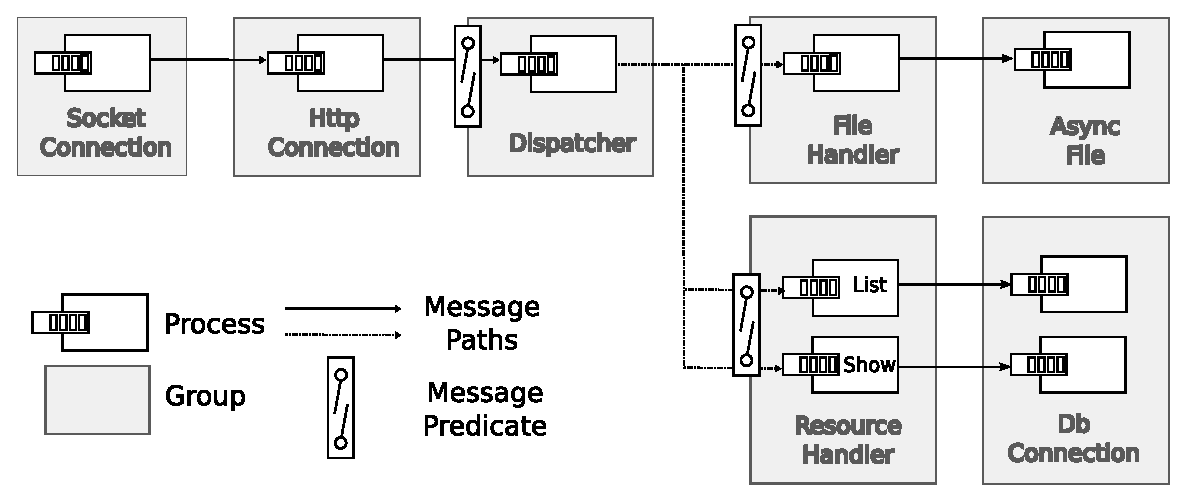
\includegraphics[width=\textwidth]{http-server.eps}
\caption{The subsystem responsible for processing HTTP connections. All of the groups contain processes of a single type except for the ``Resource Handler'' group. This group contains processes of type ``List'' for presenting a list of resources and ``Show'' for presenting detailed information about a single resource.}
\label{figure:http-server}
\end{figure*} 

Each connection to the HTTP server resulted in the creation of three processes;

\begin{itemize}
	\item a \verb+SocketConnection+ process to manage the underlying socket,
	\item a \verb+HttpConnection+ process to decode and encode HTTP messages and manage the HTTP connection state, and
	\item a \verb+Dispatcher+ that routes the HTTP requests to specific handlers based on the contents of the headers, method and uri of the request.
\end{itemize}

Each request submitted to the server results in the \verb+Dispatcher+ creating a \emph{handler} process. A handler may be responsible for delivering content from the filesystem, dynamically generating content based based on values retrieved from a database or submitting data to an external system. 

The handler will usually generate one or more processes while handling the request. For example, the \verb+FileHandler+ process creates an \verb+AsyncFile+ process while the \verb+ListDeployedResources+ process creates a \verb+DbConnection+ process. 

Some handlers will share a group if they utilize similar resources and load shedding is likely to handle these handlers similarly. However, most handlers and other other processes in the system will have a single group per process type.

Most Whirlwind applications will only place messages predicates in a few specific locations. The HTTP server defines a message predicate on the \verb+Dispatcher+ group and on each of the handler groups. 

If a message predicate attached to a handler group rejects a message then the dispatcher may attempt to send a less resource intensive request to the handler. Figure~\ref{figure:message-predicate} presents a scenario where the \verb+FileHandler+ group rejects a request for a high resolution image and a medium resolution image before accepting a request for a low resolution image. 

\begin{figure}[htbp]
\centering
TODO
%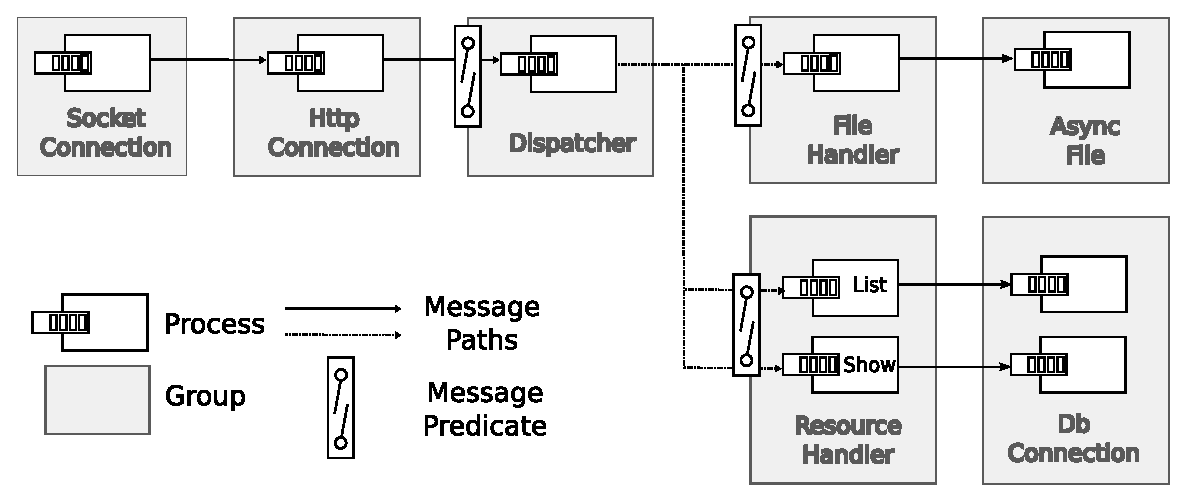
\includegraphics[width=\linewidth]{http-server.eps}
\caption{TODO}
\label{figure:message-predicate}
\end{figure}

If the message predicate attached to the \verb+Dispatcher+ group rejects a message then the \verb+HttpConnection+ sending the message will return a ``503 Service Unavailable'' response to the client and close the connection. This message predicate is only triggered when the message predicates attached to the handlers have failed to shed enough load to avoid system overload.

The HTTP server defines a single principal for each HTTP session. When a client accesses a page it is typical that several requests occur over one or more HTTP connections. The requests typically load the HTML page and supporting resources such as images. A message predicate that decides to reject messages should either reject all requests from a session or none at all, as partial loading of a page results in a poor user experience~\cite{Cherkasova:2002yb}. 

The creation of a new handler for every request rather than handler reuse is deliberate. This design results in all the processes in Figure~\ref{figure:http-server} being  associated with a single principal thus allowing consistent treatment by message predicates across the whole system.

The prioritization of principals takes into account whether the session is for an authenticated user and if the user is in the \emph{admin} role. Administrators are given the highest priority as they need to be able to view the status of the system at anytime, even if the system is overloaded while unauthenticated users are given the lowest priority.

\section{Evolution of the Framework}

Whirlwind has gone through 5 major revisions. The initial version was primarily focused on effective overload management. The following three revisions were attempts to remove sources of bugs that were revealed once the system was put into production. The latest version focused on improving performance.

\subsection{Whirlwind v1.0}

Whirlwind v1.0 was an event--driven architecture that decomposed the application into a network of stages connected with request queues. Each stage was serviced by a pool of threads. Each thread continuously looped, retrieving batches of events from the request queue and passed them to an event handler. Event handlers could be stateless and shared across all threads. The event handlers could also be stateful and instantiated once for each thread or event. The thread pool size and batch size were adaptively tuned to maximize throughput. 

Whirlwind v1.0 was heavily influenced by the SEDA~\cite{welsh03Adaptive} but adapted to use modern JVM technologies such as the Java Management eXtensions (JMX) and Java's New I/O (NIO) toolkit. The implementation was complimented with an extensive automated test suite. 

\subsection{Whirlwind v2.0}

SEDA did not provide any explicit mechanisms for protecting shared state from other threads accessing it, either within a single stage or across stages. During the first fire season, several faults were revealed that were traced to poorly accessed shared state.

Whirlwind v2.0 attempted to address this concern by encapsulating shared state in \emph{elements}. Some elements allowed multiple concurrent threads while \emph{sequential} elements only allowed one thread access at any one time. The concurrency constraints on elements were enforced by a byte code validator. The design of \emph{elements} meant that stateful event handlers were no longer necessary.

It should be noted that scheduling decisions across groups were no longer isolated. One stage could acquire a lock and block progress of a thread in another stage. Whirlwind v2.0 also removed event batching as we were unable to reproduce any measurable performance benefit.

\subsection{Whirlwind v3.0}

Whirlwind v2.0 did not guarantee any particular event ordering. Multiple threads could be attempting to delegate event handling to a single element at any one time and the ordering is determined by the JVM or operating system. Mid fire season, the hardware platform was upgraded to 16 processors which increased the frequency of out--of--order event processing and exposed several bugs with some elements ability to handle out--of--order events. 

Whirlwind v3.0 addressed this problem by adding a local FIFO queue to \emph{sequential} elements. Each time an element was scheduled it performed event handling for the next event. As non--sequential elements were not widely used they were removed, effectively transforming Whirlwind into an implementation of the actor model of concurrency. This change cascaded through the system allowing the removal of event handlers and enhancing the adaptive algorithm used to manage the thread pool size. 

\subsection{Whirlwind v4.0}

During the preceding fire season, a crash occurred as a result of accidental state sharing between elements. To address these concerns two changes were made to Whirlwind; the Erlang model of fault propagation and recovery was incorporated, and the byte code validator was enhanced to enforce isolation properties. The other major change was one of terminology; elements became processes, events became messages and stages became groups.

To enforce isolation properties of the messages, the byte code validator required that developer annotate the messages. The validator used the annotations combined with rules and heuristics to enforce the isolation constraints. The messages and all transitively referenced values needed to be either; immutable, a process or have ownership transferred from the source to destination processes. The byte code validator in many ways resembled a less capable, more ad--hoc version of the Kilim byte code weaver~\cite{Srinivasan:08:Kilim}.

\subsection{Whirlwind v5.0}

No faults were detected when Whirlwind v4.0 was deployed so the latest revision focused on performance. This resulted in the introduction of custom schedulers and principals. Custom schedulers allowed the development of application or context specific schedulers. This introduced other mechanisms to manage overload response. Principals came about as the categorization and prioritization code was being duplicated between message predicates and schedulers.

The byte code validator was removed in this version as it added significant overhead to developing Whirlwind--based services. It is unknown whether applying a more sophisticated validator as appeared in Kilim would have mitigated the cost.

\subsection{Reflections on the Evolution}

It is interesting that the evolution of Whirlwind drove it towards the actor model of concurrency. Initially the author was a strong advocate of event--driven architectures even in the context of multiple processors. Several attempts were made in an attempt to \emph{fix} this model in Whirlwind through techniques such as event coloring~\cite{Dabek02EventDriven} but with little practical success. 

The demands of deploying the code into a production environment where both failures and poor performance were costly drove the framework away from using shared memory. Forcing the process to handle messages sequentially in a FIFO order proved to result in dramatically simplified code for the process, fewer bugs and no measurable performance degradation.

\section{Related Work}

Whirlwind is an implementation of the actor model of concurrency based on the JVM that includes load management and fault management primitives. While it incorporates aspects of existing work it is most strongly related to the work on SEDA, Erlang and Kilim. 

Whirlwind incorporates load protection primitives from SEDA, namely cohort scheduling and message predicates. Whirlwind also includes fault management primitives and a supervisor library inspired by similar elements in Erlang. Whirlwind, SEDA and Kilim are all JVM based while Erlang uses a specialized virtual machine.

Whirlwind eschews the shared memory model of SEDA and assumes processes are isolated and share no state. Unlike Kilim and Erlang, ensuring the isolation of processes is partially the responsibility of the developer. A developer can inadvertently or deliberately share state between processes but in such a scenario, Whirlwind assumes that the developer knows what they are doing. 

At least one Whirlwind application made use of this ``feature'' and used an existing in--memory database that used fine grain locking to mediate access to the shared state access. All processes that accessed the shared state were placed in a single group. The processes were also linked so that if any failed, they all failed and were restarted.

In SEDA, events about a single subject can be handled concurrently and out--of--order while in Whirlwind messages are sequential and in a FIFO order. Both Kilim and Erlang handled messages sequentially but Erlang can choose to receive messages out of order.

None of SEDA, Erlang or Kilim allowed configuration of custom schedulers and no framework that we are aware of incorporates the principal abstraction. Only SEDA incorporates adaptive concurrency level.

Kilim and Erlang are independent threads of execution and can store state on the stack in between messages. Whirlwind and SEDA must explicitly store any continuation state in the process as they use a callback model and are have the message or event handling code invoked when a message or event arrives.

\section{Future Work}

There are two major changes planned for the next version of Whirlwind. The first change is to support Kilim~\cite{Srinivasan:08:Kilim} or Kilim--like processes executing on top of the Whirlwind runtime. The second is to investigate the possibility of dynamically organizing processes into groups at runtime.

\subsection{Kilim integration}

Kilim has two main advantages over the current Whirlwind process implementation. Firstly, Kilim enforces the isolation constrains through a byte code validator. Earlier versions of Whirlwind attempted this with limited success. 

Secondly, Kilim processes are lightweight threads that use automatic stack management~\cite{Adya02Cooperative} to maintain continuation data between handling messages. 
Whirlwind processes currently use complex state machines and manual stack management to achieve the same effect. Kilim attempts to optimize saving and restoring stack state when a process is paused or resumed. The degree of overhead is related to the number of frames on the stack when the process is paused or resumed. Experience with existing Whirlwind applications suggest that a paused process will only have a small number of active frames. The expectation is that the small performance degradation is acceptable tradeoff for certain classes of process.

\subsection{Automatic grouping}

Simple heuristics combined with annotations and runtime instrumentation can automate the organization of processes into groups. Using automated grouping of processes will reduce the level of complexity for developing Whirlwind based applications. As groups are likely to be created on demand, processes will need to support migration from one group to another.

A typical heuristic would be to create a group when a large number of processes of a single type are instantiated. The processes are likely to have a high degree of code locality and with large numbers the system could take advantage of cohort scheduling making these processes an ideal group.

Annotations could be added to the processes to provide hints to the runtime system to guide grouping. The annotations would indicate the resource and concurrency requirements of the processes. Where annotations were not sufficient for the runtime to group processes appropriately, the developer could fall back on manual group configuration.

Automatic grouping would likely lead to the decoupling of the message predicate from the group. The message predicate is something that the developer will likely want to attach to specific sets of processes or even message flows between specific sets of processes.

\section{Conclusions}

Whirlwind demonstrates an architecture for building high--concurrency Internet services with overload protection and fault tolerance. Whirlwind is a synthesis of existing techniques put to the test in production environments for 5 years, in a context where there is a high cost for failure or poor performance. Whirlwind managed to withstand extreme loads as a result of Victoria's worst fire season in 2009.

The programming model introduces the principal abstraction. This centralizes the categorization and prioritization of requests and allows past work in scheduling and load shedding to be examined in a unified framework.

Whirlwind also demonstrates an approach to incorporating existing load management techniques into a framework based on the actor model of concurrency. Flexible scheduling, cohort scheduling and message predicates proved to be useful additions.

\bibliographystyle{IEEEtran}
\bibliography{references}

\end{document}